%Autoren: Julian Uebe, Jan Sollmann
\nsecbegin{Ziel des Sprints}
Dieser Sprint ist ausschließlich dazu gedacht, im Verlauf des ersten Sprints identifizierte und noch nicht behobene Bugs zu entfernen. Es wurden bewusst keine neuen User-Stories (für den Benutzer) im Sprint-Backlog definiert. Der Fokus liegt darauf, die im ersten Sprint geschaffene Basis noch einmal zu stabilisieren.
\nsecend

\nsecbegin{User-Stories des Sprint-Backlogs}
\nsecbegin{Reduzierung von Bugs}
Als Softwarearchitekt und Product Owner wünschen wir uns, dass möglichst wenige Bugs auftreten, um die spätere Weiterentwicklung und damit die uneingeschränkte Funktionalität des Produkts nicht zu gefährden.
\nsecend
\nsecend % {User-Stories des Sprint-Backlogs}

\nsecbegin{Zeitliche Planung}
\begin{figure}[hbtp]
\centering
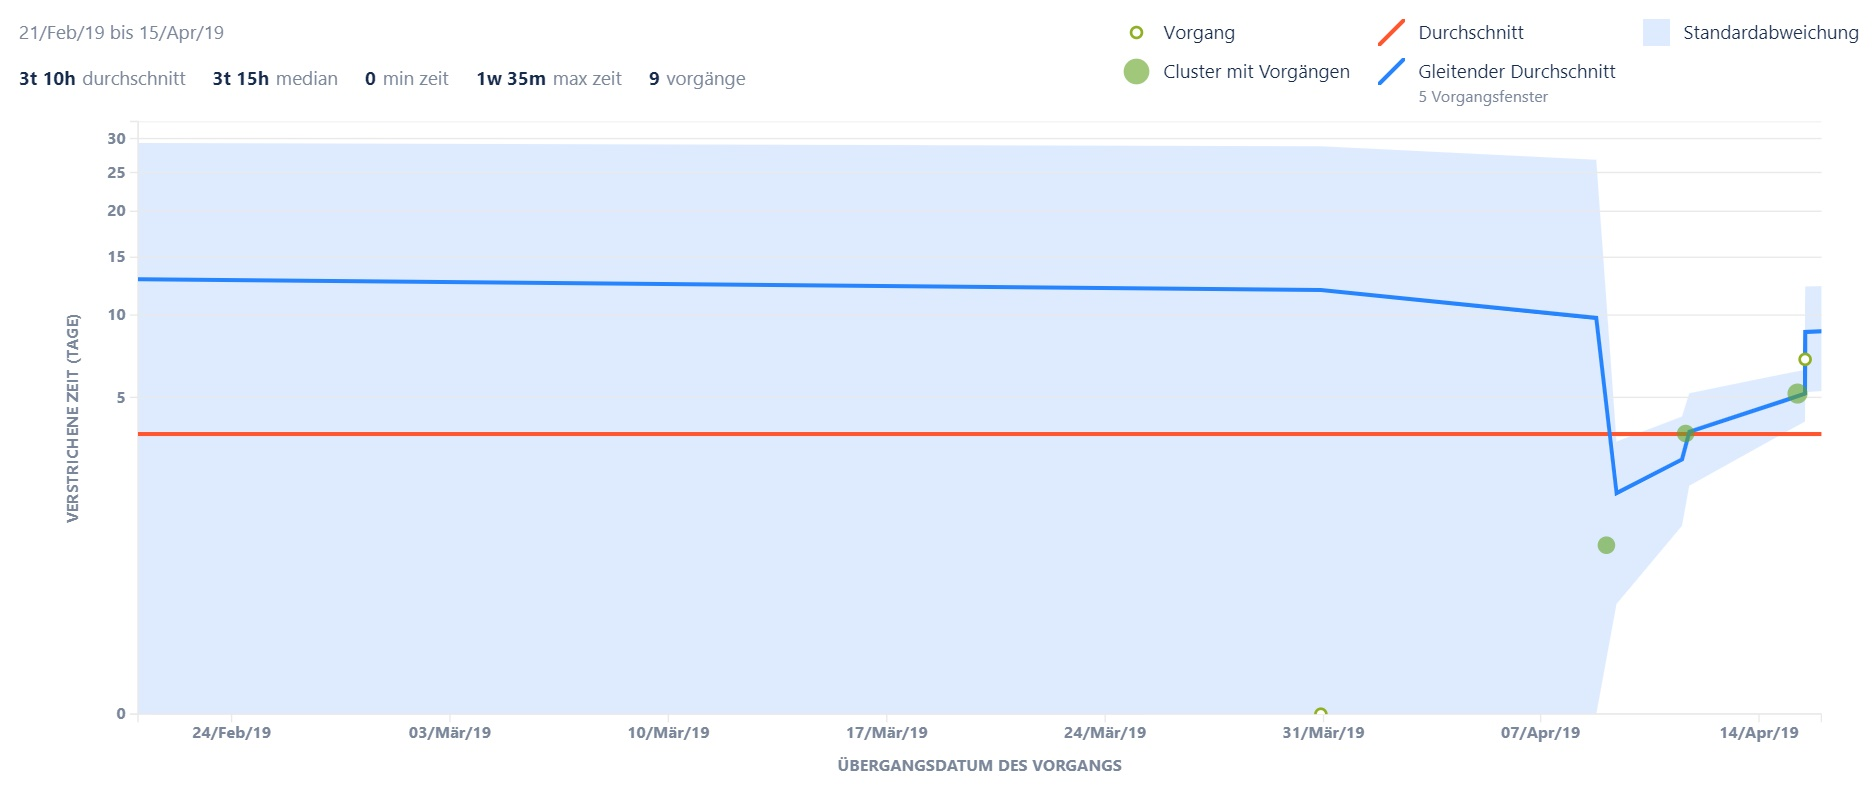
\includegraphics[width=\textwidth]{Bilder/diagram_sprint2}
\caption{Kontroll-Diagramm für Sprint 2}
\end{figure}
\nsecend%Zeitliche Planung

\nsecbegin{Liste der durchgeführten Meetings}
\begin{itemize}
\item Planning-Meeting (21.02.2019)
\item Zwischen-Meeting (08.04.2019)
\item Zwischen-Meeting (11.04.2019)
\item Review-Meeting (15.04.2019)
\end{itemize}
\nsecend%Liste der durchgeführten Meetings

\nsecbegin{Ergebnisse des Planning-Meetings}
Der zweite Sprint wird zeitlich in der letzten Woche der Semesterferien begonnen und bis zum Ende der ersten Woche der Vorlesungszeit gehen. Dies wurde mit den Teammitgliedern besprochen. Hauptziel des Sprints ist ein sauberer Stand, mit dem ab dem kommenden Sommersemester weitergearbeitet werden kann.
\nsecend

\nsecbegin{Aufgewendete Arbeitszeit pro Person$+$Arbeitspaket}
\begin{longtable}{|p{4cm}|l|l|l|l|l|}
        \hline
        Arbeitspaket & Person & Start & Ende & h & Artefakt\\
        \hline
        Testdaten & Marian Geissler   & 06.04.2019 & 15.04.2019 & 2 &  \\ \hline
        Logger & Patrick Otte   & 08.02.2019 & 08.04.2019 & 12 & LogMain.java \\ \hline
        Output & Patrick Otte   & 11.04.2019 & 15.04.2019 & 3 & OutputPUML.java \\ \hline
        Konsole & Johann Gerhardt   & 14.04.2019 & 14.04.2019 & 1 & Console.java \\ \hline
        Java-Parser & Michael Lux   & 30.03.2019 & 30.03.2019 & 14 & ParserJava.java\\ \hline
        GUI & Jan Sollmann  & 01.04.2019 & 06.04.2019 & 5 & GUI\_SWT.java \\ \hline
        GUI & Julian Uebe  & 21.02.2019 & 15.04.2019 & 7 & SWT-Tool \\ \hline
        Code-Collector & Elisabeth Schuster  & 07.02.2019 & 14.04.2019 & 5.5  & CodeCollector.java \\ \hline
        Profiler & Elisabeth Schuster  & 10.04.2019 & 26.04.2019 & 7  & Profiler \\ \hline
       Java-Parser & Jona Meyer  & 30.03.2019 & 30.03.2019 & 7 & ParserJave.java \\ \hline
        Code-Collector & Leo Rauschke  & 07.04.2019 & 14.04.2019 & 5.75 & CodeCollector.java \\ \hline
        Profiler & Leo Rauschke  & 09.04.2019 & 29.04.2019 & 3 & Profiler\\ \hline
        Output & Tore Arndt  & 11.04.2019 & 15.04.2019 & 5 & OutputPUML.java\\ \hline
        
        
\end{longtable}     
\nsecend

\nsecbegin{Konkrete Code-Qualität im Sprint}
Die Codequalität ist etwas besser geworden. Wobei hin und wieder durchaus noch massive Unschönheiten bemängelt werde müssen.
\nsecend

\nsecbegin{Konkrete Test-Überdeckung im Sprint}
Die Testüberdeckung ist auf 40,6\% gesunken.
\nsecend

\nsecbegin{Ergebnisse des Reviews}
\begin{table}[H]

\begin{tabularx}{\textwidth}{ |l|l|X| }
\hline
\textbf{Klasse} & \textbf{Methode} & \textbf{Anmerkungen}\\
 \hline
 
 Testdatensatz & komplett & zukünftig als automatischer Ausgabe-Test\\ \hline
 GUI\_SWT.java & komplett & wird durch Swing-GUI ersetzt\\ \hline
 CodeCollector & Pfadbehandlung & Funktioniert nun auch unter Windows\\ \hline
 CodeCollector & einlesen & Funktioniert\\ \hline
 ParserJava.java & buildTree & Es bestehen weitherhin Bugs\\ \hline
 Alle & komplett & Unit-Tests für das ganze Programm folgen\\ \hline
 ParserJava.java & buildTree & Erweiterung für das Erstellen von Sequenzdiagrammen\\ \hline
 GUI\_SWT.java & createContents, runPUML & Ausgabe für Sequenzdiagramme muss implementiert werden\\ \hline
 
%Console & showConsole & Pfad anpassen \\
\hline
\end{tabularx}
\end{table}

\nsecend%Ergebnisse des Reviews

\nsecbegin{Ergebnisse der Retrospektive}
Die Retrospektive schloss mit einer positiven Bilanz. (...)
\nsecend%Ergebnisse der Retrospektive

\nsecbegin{Abschließende Einschätzung des Product-Owners}
In diesem Sprint wurden einige kritische Bugs behoben und somit User Stories des letzten Sprint-Backlogs noch vervollständigt. Zu hoffen bleibt trotzdem, dass in allen folgenden Sprints auch neue Funktionalität hinzugefügt wird.
\nsecend%Abschließende Einschätzung des Product-Owners

\nsecbegin{Abschließende Einschätzung des Software-Architekten}
Der erste Meilenstein wird als erreicht angesehen, auch wenn der Parser durchaus noch Mängel enthält. Der Grundentwurf der Architektur ist vollständig umgesetzt. Da im nächsten Sprint die Sequenz-Diagramme hinzugenommen sollen, wird hier ein kleiner Umbau der Architektur notwendig sein. Die Klassen ParsingResult, welche nur Daten (unter anderem vom Typ ClassConnection) enthält wird durch XML ersetzt. Dies war von Anfang an vorgesehen, wurde aber aufgrund der höheren Komplexität bisher vermieden. Des weiteren haben wir beschlossen die Sprintdauer auf 2 Wochen zu verkürzen, um die Entwicklung zu beschleunigen.
\nsecend%Abschließende Einschätzung des Software-Architekten

\nsecbegin{Abschließende Einschätzung des Team-Managers}
Insgesamt kann positiv herausgehoben werden, dass sich die Teammitglieder geschlossen dazu bereit erklärten, Teil ihrer Semesterferien für den zweiten Sprint zu opfern. Die Motivation, das Produkt weiter voranzubringen, scheint derzeit ungebrochen.
\nsecend%Abschließende Einschätzung des Team-Managers